\section{Data Access}

The initial phase of FedCampus operates on participants' health data recorded by
the Huawei Watch Fit 2.
100 smartwatches of this model are purchased to be lent to the participants.

As a ground truth, to preserve user privacy,
the bottom line is that the raw data must not be collected.
However, in order to conduct research on the data,
our algorithms need to access the data from the smartwatch.

To deploy algorithms without collecting raw data,
we need to deploy the algorithms on users' edge devices and
access the data there.
In the natural life cycle of the collected health data,
the data are first synchronized from the participants' smartwatches to
the Huawei Health Kit~\cite{huaweihealthkit} on
their smartphone through Bluetooth.
This is important in two ways:
first, we do not need to develop any software to run on the smartwatches,
only the smartphones; second,
we require the participants to regularly conduct this synchronization process
themselves, which counts into management complexity.

We deploy different strategies to access the data from the Huawei Health Kit on
Android and iOS.
On Android, Huawei provides the Huawei Health Kit API to access the data.
On iOS, Apple restricts third-party access to private data,
and unifies such access to Apple HealthKit~\cite{applehealthkit},
so we have to first synchronize the data from the Huawei Health Kit to
the Apple HealthKit, then access the data via Apple HealthKit.

\section{The \fedcampus Application}

The major challenge of the \fedcampus Application is to
support both Android and iOS devices.
This is necessary because our participants at Duke Kunshan University are
a mix of Android and iOS users,
and we want to allow as many of them to participate as possible.
However, Android and iOS applications are incompatible,
and developing separate applications for these two platforms would be
a laborious task because
it would mean we have to maintain two separate codebases and
duplicate any changes.

To support mobile development on both Android and iOS,
we leverage the Flutter application framework.
Instead of developing two separate applications for Android and iOS,
by using Flutter,
only a single codebase is needed to for both the Android and iOS versions of
the application.
Therefore, we implement as much of the \fedcampus Application on Flutter as
possible to maximize our code reuse and minimize our development effort.

\section{Designing \fedkit}

As an overview,
\fedkit is a software development kit meticulously crafted to facilitate
federated learning seamlessly among clients operating on both Android and iOS
devices. Given the inherent limitations imposed by smartphone operating systems,
which restrict external software to function solely as "applications," our
clients, in this context, are the smartphone applications.
To effectively orchestrate and control the federated learning process,
a backend server is essential.
This server handles the scheduling of training on the clients and manages the
aggregation of machine learning models.

\subsection{Challenges in \fedkit's Design}

The design of \fedkit faces three major challenges:

The design of \fedkit confronts three significant challenges:

\begin{enumerate}
\item Cross-Platform Support:
    To tap into the potential participant pool at Duke Kunshan University,
    the \fedcampus Application needs to support both Android and iOS devices.
    This necessitates that any federated learning system integrated into it must
    also cater to both platforms. However,
    existing on-device training frameworks for smartphones typically support
    only one of these platforms. Consequently,
    we find ourselves compelled to implement machine learning models twice and
    train them separately on Android and iOS,
    which leads to the fragmentation of participant data,
    undermining the essence of federated learning.
\item Dependency on Application Updates:
    In conventional examples of machine learning on smartphones from major
    frameworks,
    the machine learning models are embedded within the applications,
    tying model updates to application updates. However,
    the process of updating applications may involve reviews by the vendor's
    application store or require user intervention,
    stripping the \fedcampus team of control and posing challenges in iterating
    machine learning models in a production setting.
\item Interdisciplinary Collaboration:
    Integrating any federated learning process into the \fedcampus Application
    demands proficiency in both mobile development for implementation and
    machine learning for the algorithm.
    These intertwined requirements means that the software developer and
    the data scientist on the \fedcampus team have to work very closely for
    any federated-learning-related features and adjustments,
    resulting in significant development overhead.
\end{enumerate}

To address the first challenge,
we have devised a cross-platform federated learning model pipeline.
This comprehensive pipeline supports the entire federated learning process,
encompassing model creation, deployment, training, and aggregation,
as detailed in Section~\ref{sec:pipeline}. For the second challenge,
our federated learning workflow empowers flexible machine learning operations
from the backend in production, as we detail in Sec.~\ref{sec:mlops}.
The overall approach addresses the third challenge by providing a user-friendly
development environment in Python. Consequently,
\fedkit allows researchers to accomplish all tasks related to machine learning
model creation and algorithm deployment using their familiar Python frameworks.

\subsection{Cross-Platform Federated Learning Model Pipeline}
\label{sec:pipeline}

While many machine learning researchers are well-versed in Python-based
frameworks like PyTorch and TensorFlow,
the challenge lies in the fact that models developed using these frameworks
generally do not run on smartphones.
Google and Apple have each devised their frameworks for machine learning tasks,
each with its model format and runtime,
rendering them incompatible with each other.

To enable cross-platform federated learning,
especially cross-platform aggregation,
we propose a pipeline comprising model conversion and unified training APIs,
illustrated in Fig.~\ref{fig:pipeline}.

\begin{figure}\begin{center}
    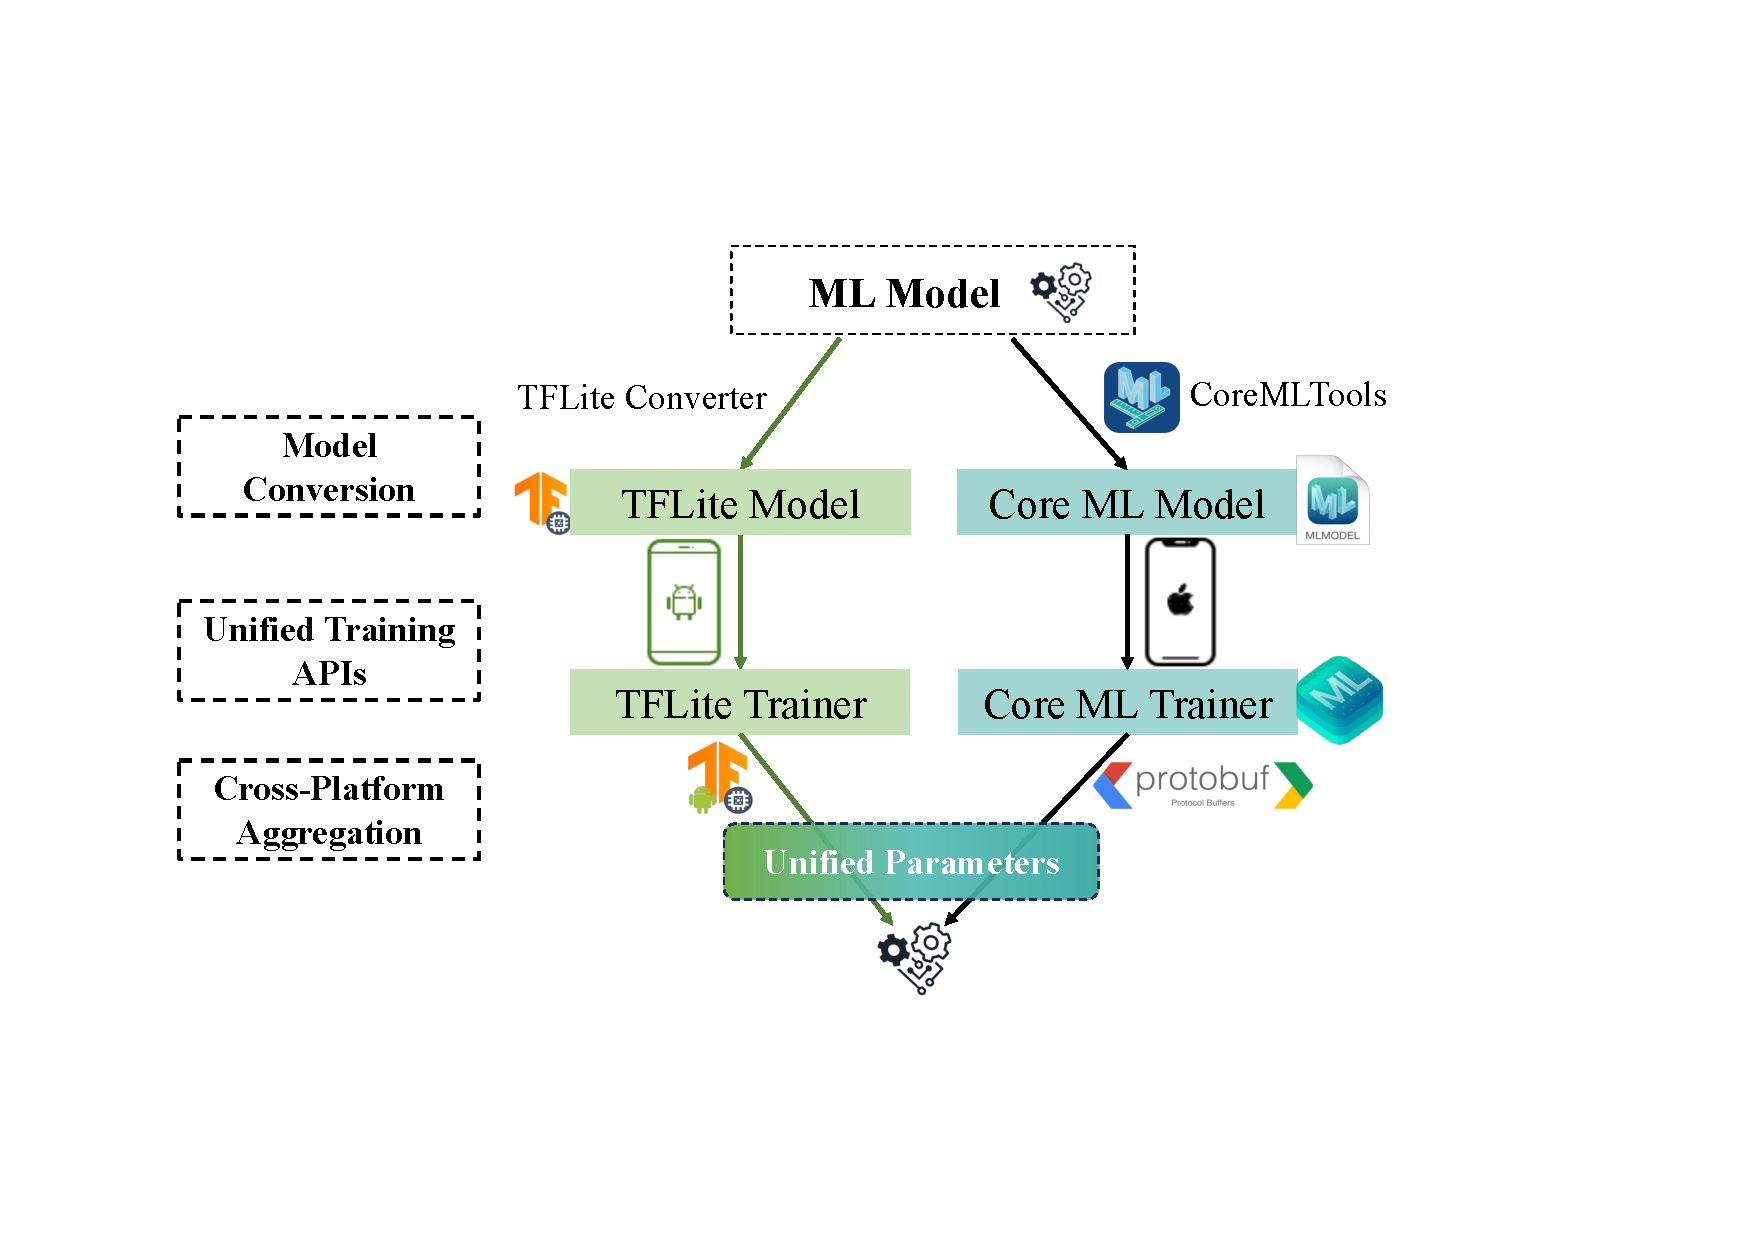
\includegraphics[width=\linewidth]{model_pipeline.pdf}
    \caption{\fedkit Model Pipeline for Cross-Platform Federated Learning.}
    \label{fig:pipeline}
\end{center}\end{figure}

\subsubsection{Model Conversion}
To create machine learning models in Python and deploy them on platform-specific
machine learning frameworks,
we initiate the process by converting models into compatible
formats---TensorFlow Lite for Android and Core ML for iOS.
Core ML follows a fixed model structure defined in the ProtoBuf format,
and provides the official converter CoreMLTools,
therefore we directly adapt both the model format and the conversion.
On the contrary,
TensorFlow Lite allows specifying custom arbitrary functionalities in the model,
and provides a Python API for model conversion.
To unify the model format and conversion process,
we standardized a model format for TensorFlow Lite and developed a compliant
TensorFlow converter.
This standardized format includes four essential federated learning methods to
train the model, perform inference, and extract and update model parameters.

\subsubsection{Unified Training APIs}
On-device training stands out as the most intricate aspect of federated learning
on smartphones due to the complexity, experimental nature,
and lack of community guidance in the involved libraries.
\fedkit simplifies this integration by providing trainers that encapsulate
on-device training libraries and expose only a minimal interface required by
federated learning.

Specifically,
\fedkit offers the TensorFlow Lite Trainer and the Core ML Trainer for training
the converted models on Android and iOS devices respectively,
utilizing OpenGL and Core ML acceleration.
Both trainers expose unified APIs for retrieving and setting model parameters,
model fitting, and evaluation.

While on Android,
these APIs invoke the TensorFlow Lite interpreter to call our standardized
methods defined in Model Conversion, on iOS,
Core ML forbids setting model parameters directly.
Since updating model parameters is a fundamental operation in federated
learning,
This limitation could have rendered federated learning impossible with Core ML.
Luckily, we were able to find a mostly undocumented workaround.
We modify the underlying ProtoBuf representations of Core ML models,
utilizing Swift code generated from relevant ProtoBuf definition files to
navigate nested model definitions and access parameters on iOS. Consequently,
our unified training APIs exhibit comparable functionality on both iOS and
Android platforms.

\subsubsection{Cross-Platform Model Aggregation}
The model aggregation step in federated learning necessitates uniform parameter
representations,
posing primary challenges in retrieving and setting model parameters for Core ML
and TensorFlow Lite. Firstly,
Core ML permits only specific layers of the machine learning models to be
updatable;
only parameters for these layers can be obtained after each round of training.
To obtain parameters for other layers,
we implement a solution using ProtoBuf manipulation,
involving recording layer information during Model Conversion and utilizing it
during training. Secondly,
the TensorFlow Lite interpreter only accepts inputs or outputs to functions as
maps from names to tensors. During Model Conversion,
we assign index-based names to each parameter layer and dynamically generate the
concrete methods that accept these arguments. During training,
we call the methods with these index-based names to access parameters.
These unified parameters enable seamless cross-platform model aggregation.

% TODO: Fit this in.
\subsubsection{On-Device Training}

The FedScale benchmark~\cite{lai2022fedscale} takes an interesting approach to
run TensorFlow on Android---it uses the Termux Application to
create a UNIX shell environment.

\subsection{Machine Learning Operations}
\label{sec:mlops}

\newcommand{\model}{$M$}
\newcommand{\fs}{$S_\mathrm F$}
In a production setting,
federated learning development encounters challenges stemming from the lack of
direct control over end devices.
\fedkit addresses this limitation by empowering researchers to deploy models and
algorithms continuously, a practice known as machine learning operations.
Leveraging our complete control of the self-hosted backend server,
\fedkit's three-step federated learning workflow facilitates continuous delivery
and training, as depicted in Fig.~\ref{fig:fl-workflow}.

\begin{figure}\begin{center}
    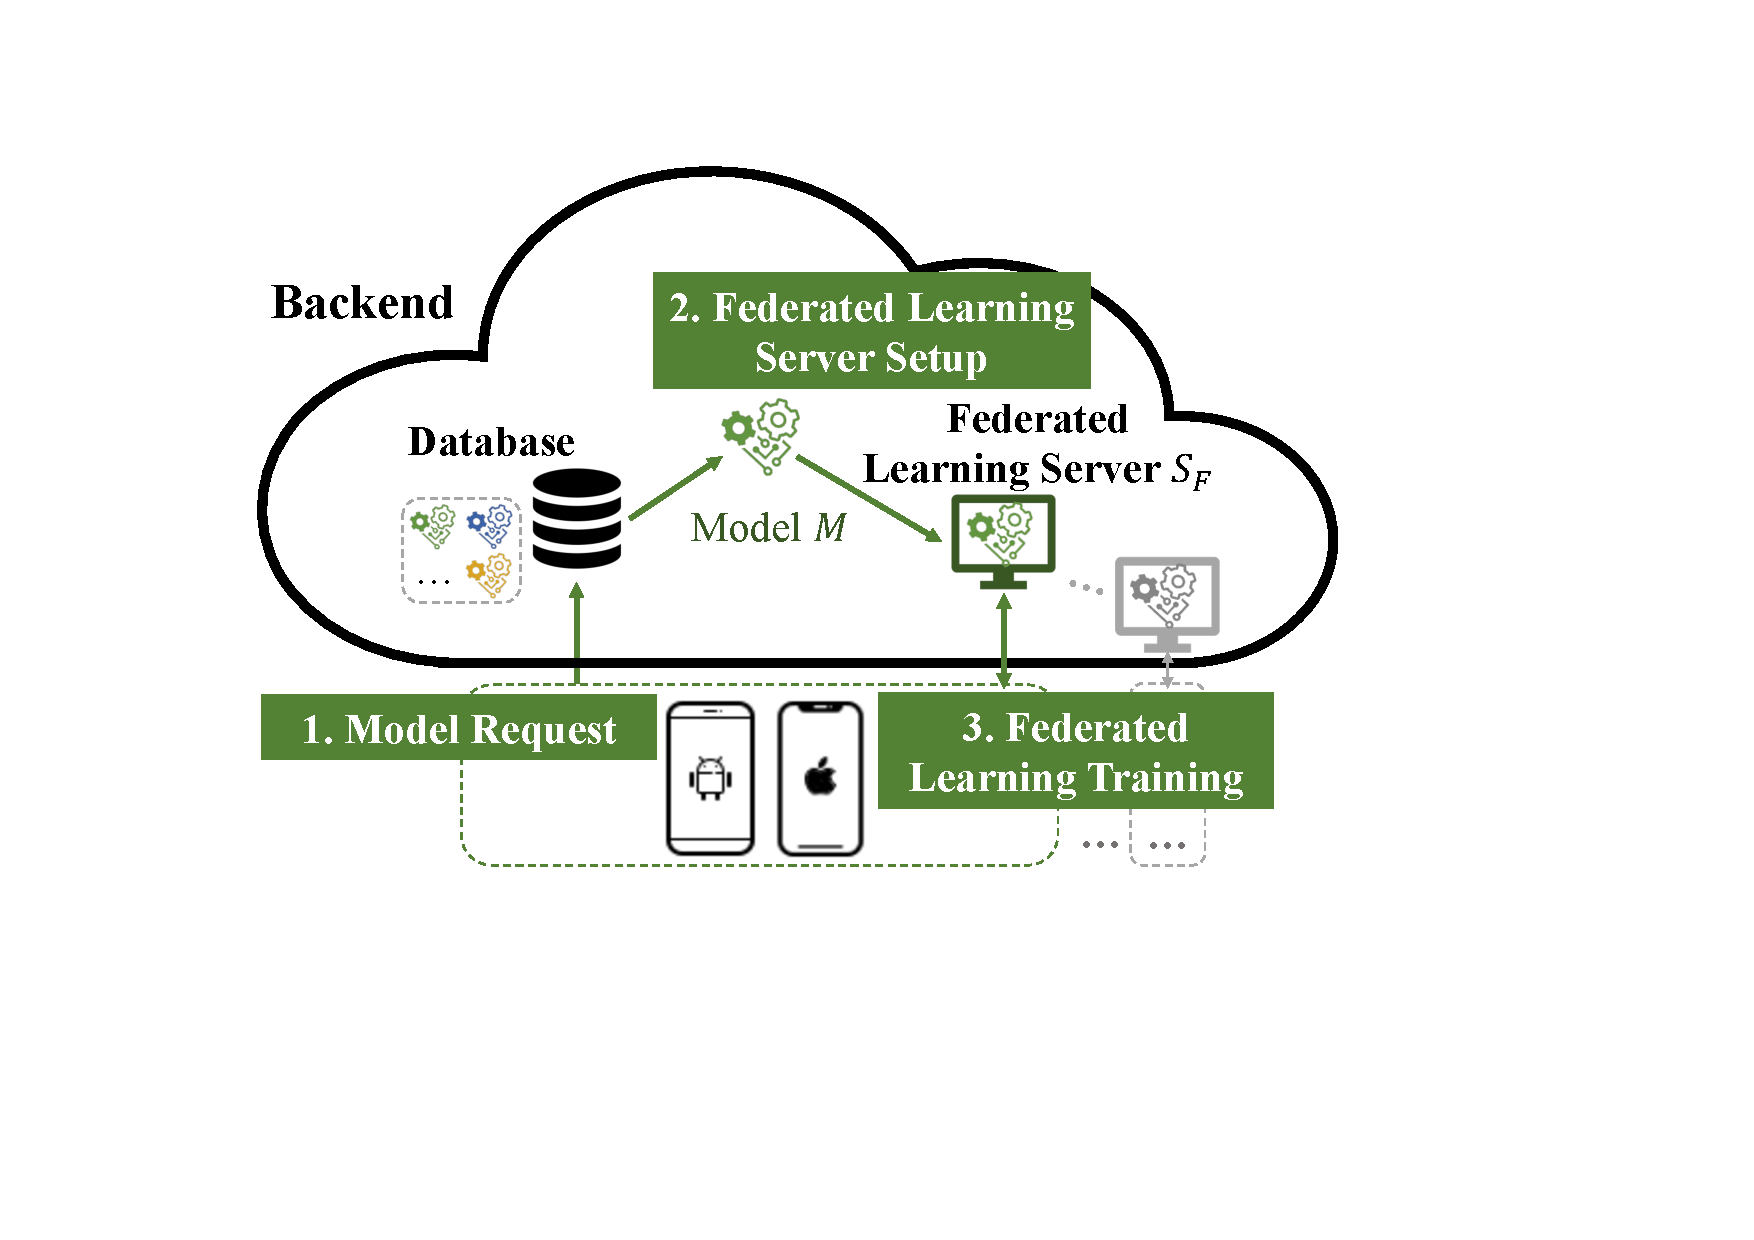
\includegraphics[width=0.7\linewidth]{fl_workflow.pdf}
    \caption{\fedkit federated learning Workflow.}
    \label{fig:fl-workflow}
\end{center}\end{figure}

\subsubsection{Continuous Cross-Platform Model Delivery}
Traditionally, models for on-device training are embedded into client apps.
However, this approach couples model delivery with app updates,
resulting in complexities when submitting apps to app stores and garnering user
adoption.

Circumventing this complexity,
\fedkit enables continuous model delivery without app updates by decoupling
models from clients through Model Request. This mechanism allows new model
deployment by uploading to the backend server. Specifically,
clients request the backend server for a TensorFlow Lite or Core ML model
aligned with their platform (Android or iOS) and training data type.
The backend server selects the appropriate model \model{}
from the database and responds with detailed model information. Consequently,
Model Request delivers the TensorFlow Lite or Core ML model file for \model{}
to clients for federated learning training.
This makes real-world mobile FL experiments feasible---instead of constantly
annoying the users by telling them to update the apps,
we can trivially iterate on the models without users noticing.

\subsubsection{Customizable Continuous federated learning Training}
\fedkit manages continuous federated learning training by enabling multiple
parallel federated learning training sessions through federated learning server
setup.
When clients request a federated learning server to train their chosen model
\model{},
the backend server either reuses a suitable federated learning server \fs{}
if it exists or spawns a new one.
Each federated learning server operates as an independent Python subprocess of
the backend server,
occupying its own port for clients to directly connect to for federated learning
training.
This dynamic approach ensures that newly delivered models can be immediately
trained with new federated learning servers without affecting ongoing ones.
Furthermore,
these federated learning servers employ the Flower federated learning
framework~\cite{beutel2020flower} for scheduling training and evaluation,
providing flexibility for federated learning algorithm customizations in Python.
With the power of our custom backend server and the Flower framework,
researchers can have fine-grained control over the entire federated learning
process by directly modifying the backend server and the federated learning
server code in Python.

Additionally, on every round of training,
the backend server records the model parameters and telemetry information,
including timing and loss.
This additional information proves invaluable for federated learning researchers
as they can closely observe and analyze the performance of their models.
